\documentclass[11pt]{article}
\usepackage[T1]{fontenc}
\usepackage{lmodern}
\usepackage[margin=1in]{geometry}
\usepackage{microtype}
\usepackage{amsmath,amssymb}
\usepackage{graphicx}
\usepackage{booktabs,tabularx,array}
\usepackage{enumitem}
\usepackage{xcolor}
\usepackage[most]{tcolorbox}
\usepackage{caption}
\usepackage{upquote}
\usepackage{needspace}
\usepackage[colorlinks=true,linkcolor=blue!50!black,urlcolor=blue!50!black]{hyperref}

\definecolor{plainbg}{HTML}{EEF4FA}\definecolor{plainframe}{HTML}{2C6FA8}
\definecolor{warnbg}{HTML}{FBF1E6}\definecolor{warnframe}{HTML}{C07020}
\newtcolorbox{plain}[1][In plain terms]{colback=plainbg,colframe=plainframe,
  fonttitle=\bfseries\small,title={#1},boxrule=0.5pt,arc=2pt,left=6pt,right=6pt,top=4pt,bottom=4pt}
\newtcolorbox{caution}[1][Watch out]{colback=warnbg,colframe=warnframe,
  fonttitle=\bfseries\small,title={#1},boxrule=0.5pt,arc=2pt,left=6pt,right=6pt,top=4pt,bottom=4pt}
\newcommand{\code}[1]{\texttt{\small #1}}
\setlist{itemsep=2pt,topsep=4pt}
\renewcommand{\arraystretch}{1.15}
\captionsetup{font=small,labelfont=bf}
\makeatletter\let\rawinput\@@input\makeatother

\title{\textbf{Simulation study results: the full design}\\[4pt]
\large 8 replicates of the \code{fitted} scenario, 1,101 subjects, 3 chains $\times$ 20,000 iterations}
\date{October 2026}
\author{}

\begin{document}
\maketitle
\vspace{-2.2em}

\begin{plain}[Summary]
We generated 8 fake ADNI cohorts from the model's own answers, refitted the model to each, and compared what it reported with what we had planted. \textbf{Overall the model recovers the truth well.} Its 95\% intervals contain the truth 121 times out of 128 for the headline quantities, which is 94.5\%, exactly what honest intervals should do. The time and rate ratios, which carry the report's ``when, not how fast'' message, show no detectable bias. It sorts accumulators from non-accumulators with an AUC of 0.95, and it confirms the README's warning about correlating posterior medians.

\textbf{One clear problem:} the APOE4 odds ratio for ever accumulating comes back about 23\% too small in every replicate, 4.10 against a true 5.32. The cause is identified: the prior on that coefficient is narrow enough to pull a large effect toward zero, and a simple formula predicts the size of the pull almost exactly. The real-data odds ratio of 5.4 is therefore probably an \emph{under}estimate. A refit with a wider prior on the susceptibility effects is the main recommendation.

With only 8 replicates, small biases cannot be detected and coverage for any single quantity is coarse. These results are preliminary in that sense, though the main finding is far outside Monte Carlo noise.
\end{plain}

%=====================================================================
\section{What was run}

\begin{center}
\small
\begin{tabular}{@{}l l@{}}
\toprule
Scenario & \code{fitted}: the truth is the shipped posterior median \\
Design & the real ADNI design: 1,101 subjects, their real visit ages and covariates \\
Fitting & 3 chains $\times$ 20,000 iterations, first third discarded \\
Replicates & 8, one per worker, about 136 minutes each \\
Results & \code{results/sim/full/rep\_fitted\_001.rds} to \code{\_008.rds} \\
\bottomrule
\end{tabular}
\end{center}

All 8 replicates finished without error. Across replicates the simulated cohorts were 71\% accumulators on average, with 62\% already progressing at the middle of follow-up and 10\% not yet started, matching the real cohort's estimated make-up.

\paragraph{Reading results from 8 replicates.} Every summary below is itself an estimate with Monte Carlo error. Two consequences matter:

\begin{itemize}
  \item \textbf{Coverage for one quantity is coarse.} It can only be 0/8 to 8/8. If the true coverage is 95\%, seeing 7 or 6 out of 8 is common: the chance of 6 or fewer is about 6\%. Pooling across quantities is far more informative, and is done in Section~\ref{sec:overall}.
  \item \textbf{Only biases larger than about 2 Monte Carlo SEs are detectable.} Each bias is reported with its Monte Carlo SE. A bias under 2 SEs is not evidence of anything.
\end{itemize}

\paragraph{Convergence.} The worst R-hat in each replicate ranged from 1.018 to 1.118. Seven replicates had every parameter at or below 1.03. Replicate 2 was the exception, with $\sigma_\delta$ at 1.118 and $\sigma_\alpha$ at 1.053. Of the 9 intervals that missed the truth, only one came from replicate 2, so the misses are not explained by poor mixing.

%=====================================================================
\section{Overall: are the intervals honest?}\label{sec:overall}

\begin{center}
\small
\begin{tabular}{@{}l r r r@{}}
\toprule
Group & Intervals & Contain the truth & Rate \\
\midrule
16 headline quantities $\times$ 8 & 128 & 121 & 94.5\% \\
10 rate-curve points $\times$ 8 & 80 & 78 & 97.5\% \\
\bottomrule
\end{tabular}
\end{center}

Both rates are consistent with 95\%. A second check standardises every error by its own posterior SD, $z = (\text{estimate} - \text{truth}) / \text{posterior SD}$. If the intervals are honest, these $z$ values behave like draws from a standard normal. For the headline quantities they have mean $-0.08$ and SD 1.08, which is close to 0 and 1. Excluding the four quantities driven by the susceptibility coefficients, they have mean 0.06 and SD 1.01.

\begin{figure}[h]
\centering
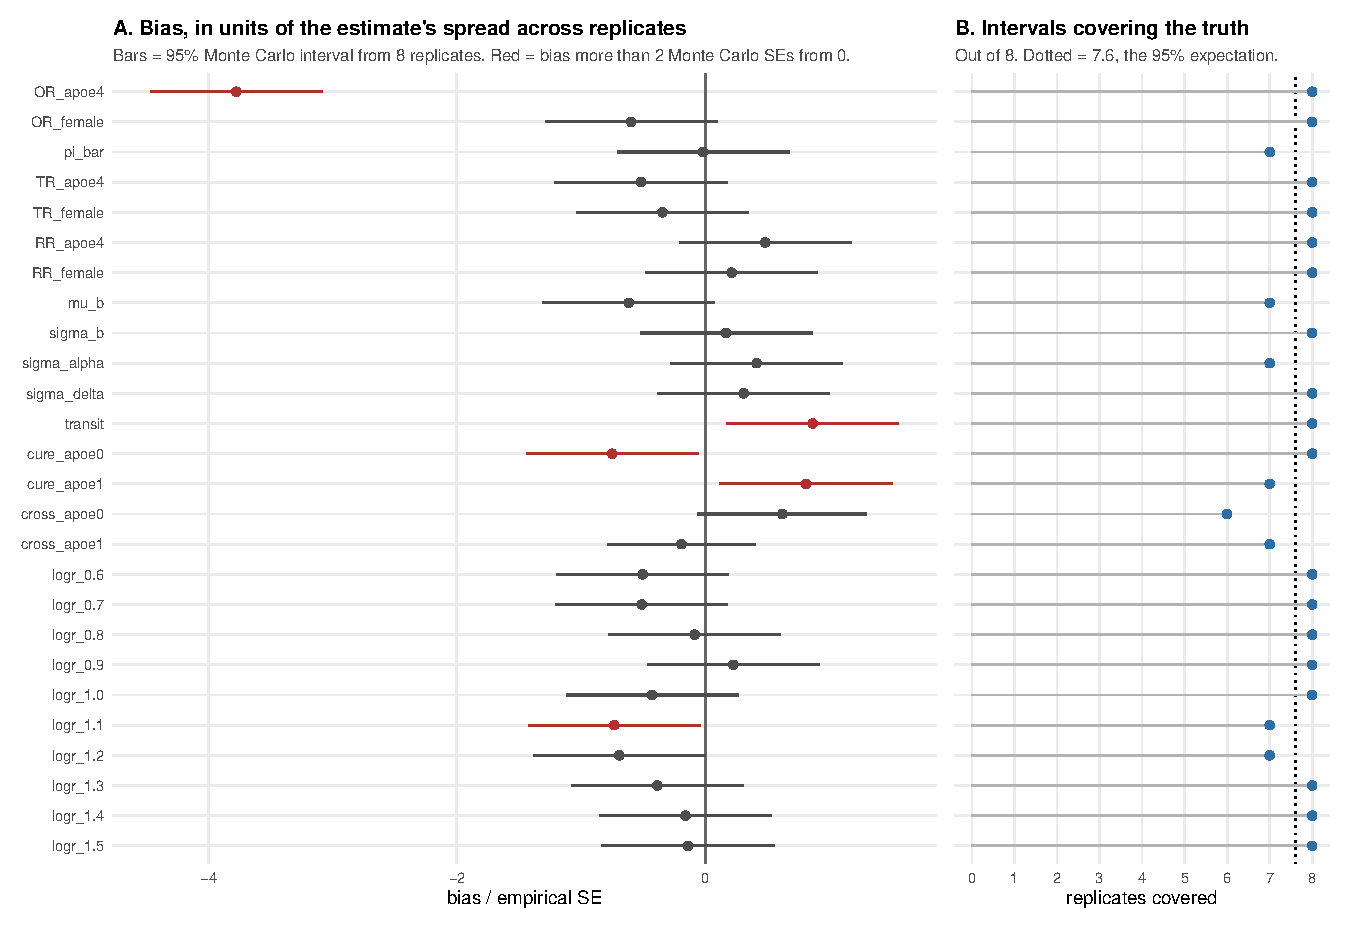
\includegraphics[width=\textwidth]{fig1_bias_coverage.pdf}
\caption{Left: each quantity's average error, scaled by how much its estimate varies across replicates, with a 95\% Monte Carlo interval. Red marks a bias more than 2 Monte Carlo SEs from zero. Right: how many of the 8 intervals contained the truth.}
\label{fig:bias}
\end{figure}

\begin{plain}
If a model says ``I'm 95\% sure'', it should be right about 95 times in 100. Across all its main answers, this model was right 121 times out of 128. It is neither overconfident nor sloppy overall. The problems are specific, and the next sections find them.
\end{plain}

%=====================================================================
\section{Quantity by quantity}

\begin{center}
\small
\begin{tabular}{@{}l r r r r r r r@{}}
\toprule
Quantity & Truth & Mean est. & Bias & MCSE & Rel.\ \% & Covered & SD ratio \\
\midrule
\rawinput tab_perf.tex
\bottomrule
\end{tabular}
\end{center}
{\small Bold bias: more than 2 Monte Carlo SEs from zero. SD ratio: the average posterior SD divided by the spread of the estimates across replicates. Near 1 means the intervals are the right width; above 1, wider than needed; below 1, too narrow. With 8 replicates each ratio is uncertain by roughly $\pm 25\%$.\par}

\subsection{The ``when'' and ``how fast'' effects are recovered}

The time ratios and rate ratios for APOE4 and sex all have biases well within Monte Carlo error, and all 32 of their intervals contained the truth. The APOE4 rate ratio is estimated at 1.12 on average against a true 1.09, a difference of 1.4 Monte Carlo SEs, so not distinguishable from zero. In the world the model describes, it estimates both the onset effect and the speed effect without mixing them up.

This scenario cannot show whether the model would wrongly report a \emph{speed} effect as an \emph{onset} effect. That is what the \code{rate\_only} scenario tests, and it has not been run yet.

\subsection{The susceptibility odds ratio is pulled toward 1}

The APOE4 odds ratio for ever accumulating averages 4.10 against a true 5.32, too low in all 8 replicates. The bias is 10.7 Monte Carlo SEs from zero, so it is certainly real. The intervals still contain the truth every time, because they are wide; Figure~\ref{fig:shrink}A shows the truth sitting near the top of every interval.

\paragraph{The cause is the prior.} The APOE4 susceptibility coefficient $\varphi_2$ has a Normal(0, $0.5^2$) prior. On the log-odds scale the truth is 1.67, which is 3.3 prior SDs from zero. Under a normal approximation, a prior with SD $s_0$ and a posterior with SD $s$ pulls the estimate toward zero by about $w \times \text{truth}$, where $w = s^2 / s_0^2$ is the prior's share of the information. The table applies this to all six covariate effects.

\begin{center}
\small
\begin{tabular}{@{}l r r r r r r@{}}
\toprule
Effect & Prior SD & \shortstack[r]{Truth in\\prior SDs} & \shortstack[r]{Posterior\\SD} & \shortstack[r]{Prior\\weight $w$} & \shortstack[r]{Predicted\\bias} & \shortstack[r]{Observed bias\\(MCSE)} \\
\midrule
\rawinput tab_shrink.tex
\bottomrule
\end{tabular}
\end{center}

For the APOE4 odds ratio the predicted pull is $-0.295$ on the log scale, and the observed pull is $-0.262 \pm 0.029$. The formula accounts for essentially all of it. For every other effect the prior's weight is small or the truth is close to zero, so the predicted pull is negligible, and the observed biases are all within 2 Monte Carlo SEs of it.

\begin{figure}[h]
\centering
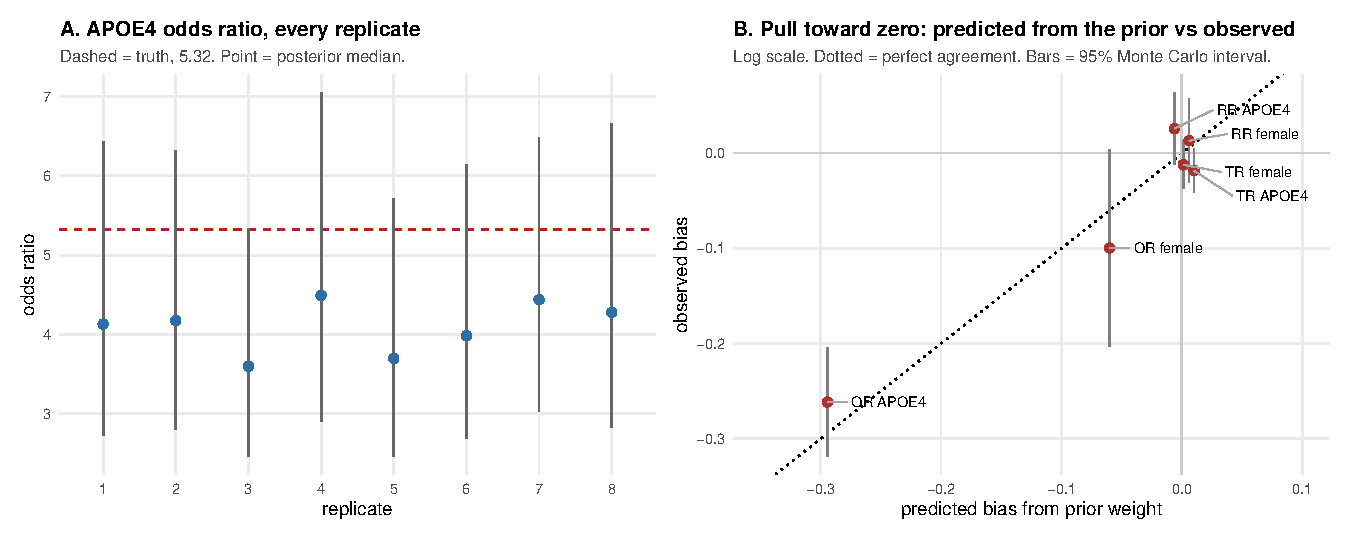
\includegraphics[width=\textwidth]{fig2_shrinkage.pdf}
\caption{Left: the APOE4 odds ratio in each replicate; every posterior median lies below the truth. Right: the pull toward zero that the prior predicts against the pull observed, for all six covariate effects on the log scale. Only the APOE4 odds ratio is pulled noticeably, and by the predicted amount.}
\label{fig:shrink}
\end{figure}

\paragraph{Knock-on effects.} Shrinking the APOE4 odds ratio toward 1 pulls the two groups' cure fractions toward each other. The never-accumulate fraction is underestimated for non-carriers, 0.380 against 0.407, and overestimated for carriers, 0.132 against 0.114. Both biases are just over 2 Monte Carlo SEs. The female odds ratio is pulled the same way, 1.36 against 1.49, but at 1.7 Monte Carlo SEs that is not individually detectable.

\paragraph{What this means for the real data.} The real-data estimate, 5.36 in the 80k run, was produced by the same prior. If the pull is roughly proportional, so that the estimate is about $(1 - w)$ times the truth on the log scale, the APOE4 odds ratio implied by the data alone would be around $\exp(1.68 / 0.82) \approx 7.7$. Treat that number only as an indication of direction and size; the honest way to find out is to refit with a wider prior. The direction matters for the report: the APOE4 effect on susceptibility is, if anything, \emph{understated}.

\begin{plain}
A prior is the model's starting belief before it sees data. Here the starting belief was ``APOE4 probably doesn't change the odds of ever accumulating by much''. The real effect is large, and the data could not fully overrule that belief, so the model's answer ends up about a quarter too small. The conclusion that APOE4 strongly affects who accumulates still stands. If anything, the true effect is bigger than reported.
\end{plain}

\subsection{Smaller findings}

\begin{itemize}
  \item \textbf{Transit budget.} Estimated at 11.4 years against a true 10.7, a 6\% overestimate at 2.4 Monte Carlo SEs. The intervals are wide, with an SD ratio of 1.7, and all 8 contain the truth, so this does not affect inference.
  \item \textbf{Onset intercept $\gamma_1$.} Biased by $-0.022$ on the log scale, 5.4 Monte Carlo SEs, which shortens the typical time from age 25 to departure by about 2\%, under one year, too small to matter. Its intervals are about three times wider than the spread of its estimates, so they are conservative.
  \item \textbf{Crossing age for non-carriers.} Estimated 0.9 years late on average, at 1.8 Monte Carlo SEs, with 6 of 8 intervals covering. Part of this is built into the comparison: the estimate averages over subjects the model classifies as accumulators, while the truth averages over the true accumulators. Worth watching as replicates are added.
  \item \textbf{The rate curve.} Recovered closely across the range (Figure~\ref{fig:curve}). It is slightly low around 1.1 to 1.2 SUVR, about 7\%, at about 2 Monte Carlo SEs, with 7 of 8 intervals covering at those two points.
  \item \textbf{Interval widths.} Most SD ratios are between 0.8 and 1.4, which is right given the noise from 8 replicates. Quantities strongly influenced by the prior, such as the APOE4 odds ratio, the transit budget and the ends of the rate curve, have ratios of 1.7 to 2.8; their intervals are conservative. The crossing ages have ratios of 0.68 and 0.76, so their intervals may be slightly too narrow, a point to recheck with more replicates.
\end{itemize}

\begin{figure}[h]
\centering
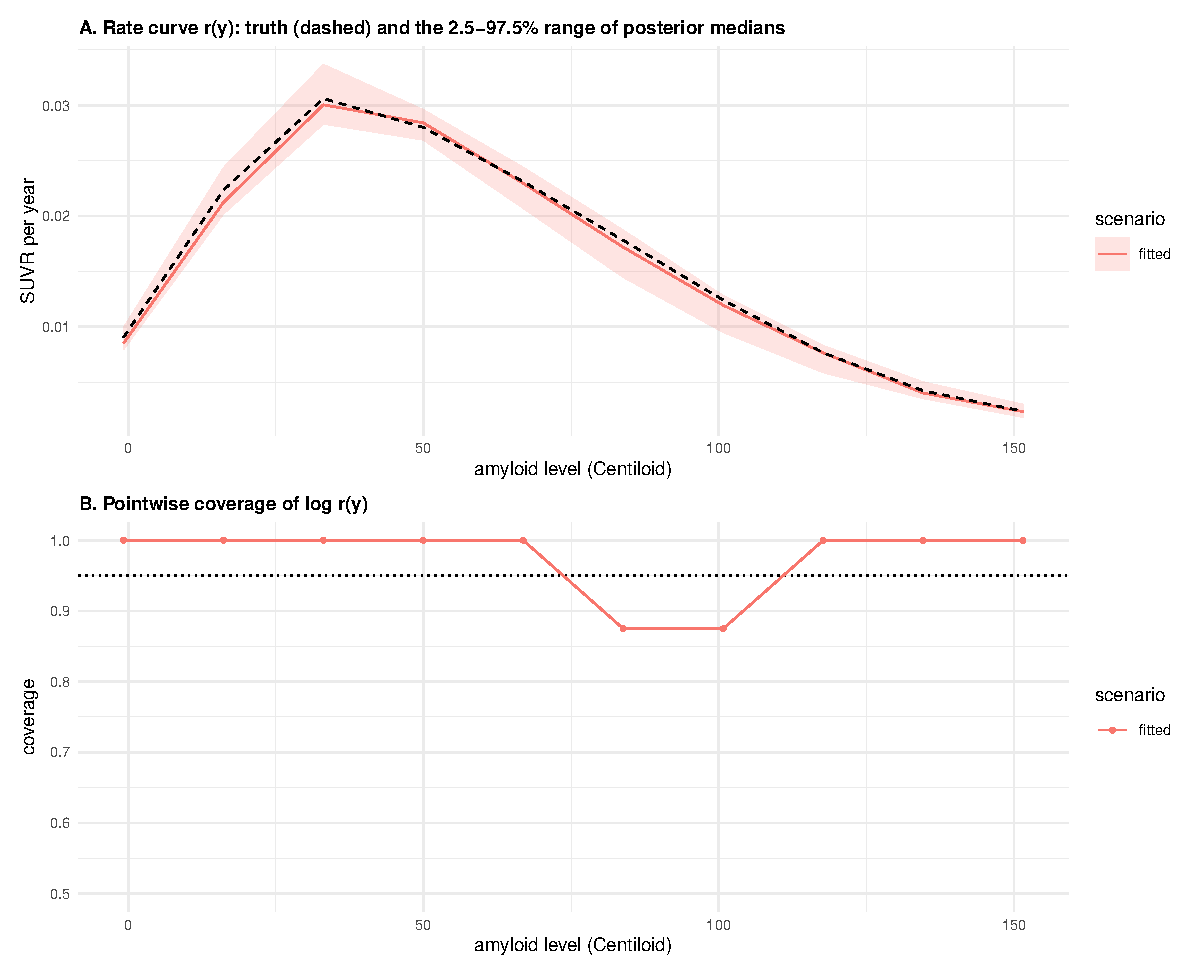
\includegraphics[width=0.82\textwidth]{../figures/sim/full/fig_sim3_rate_curve.pdf}
\caption{Top: the true rate curve (dashed) and the range of the 8 estimated curves. Bottom: how often the interval at each level contained the truth.}
\label{fig:curve}
\end{figure}

%=====================================================================
\section{Individual subjects}

\begin{center}
\small
\begin{tabularx}{\textwidth}{@{}X l@{}}
\toprule
Measure & Mean [min, max] over the 8 replicates \\
\midrule
\rawinput tab_subj.tex
\bottomrule
\end{tabularx}
\end{center}

\begin{itemize}
  \item \textbf{Membership.} The model separates true accumulators from non-accumulators well, with an AUC of 0.95. Subjects who will accumulate but have not started (state L) get an average probability of 0.63, between the cured at 0.30 and the progressing at 0.93, which is what their flat scans should produce.
  \item \textbf{Departure age, people who have started.} Essentially unbiased, with a typical error of about 6 years and 94\% coverage. Six years is the honest precision for a person seen over a four-year window of a twenty-year process.
  \item \textbf{Departure age, people who have not started.} Estimated about 7 years too \emph{early} on average, with a typical error of 10.6 years and 90\% coverage. Their scans say only that nothing has happened yet, so the estimate leans on the population distribution of onset ages. Individual onset-age estimates for currently flat subjects should not be over-interpreted.
  \item \textbf{Speed.} Typical error 0.36 on the log scale, with 93\% coverage.
  \item \textbf{The correlation trap is confirmed.} Departure age and speed are independent in every simulated cohort. Correlating the per-subject posterior medians nevertheless gives $-0.48$ on average. Computing the correlation within each posterior draw gives $-0.04$. This reproduces the README's warning on fresh data: the correlation of medians is manufactured by the estimator.
\end{itemize}

\begin{figure}[h]
\centering
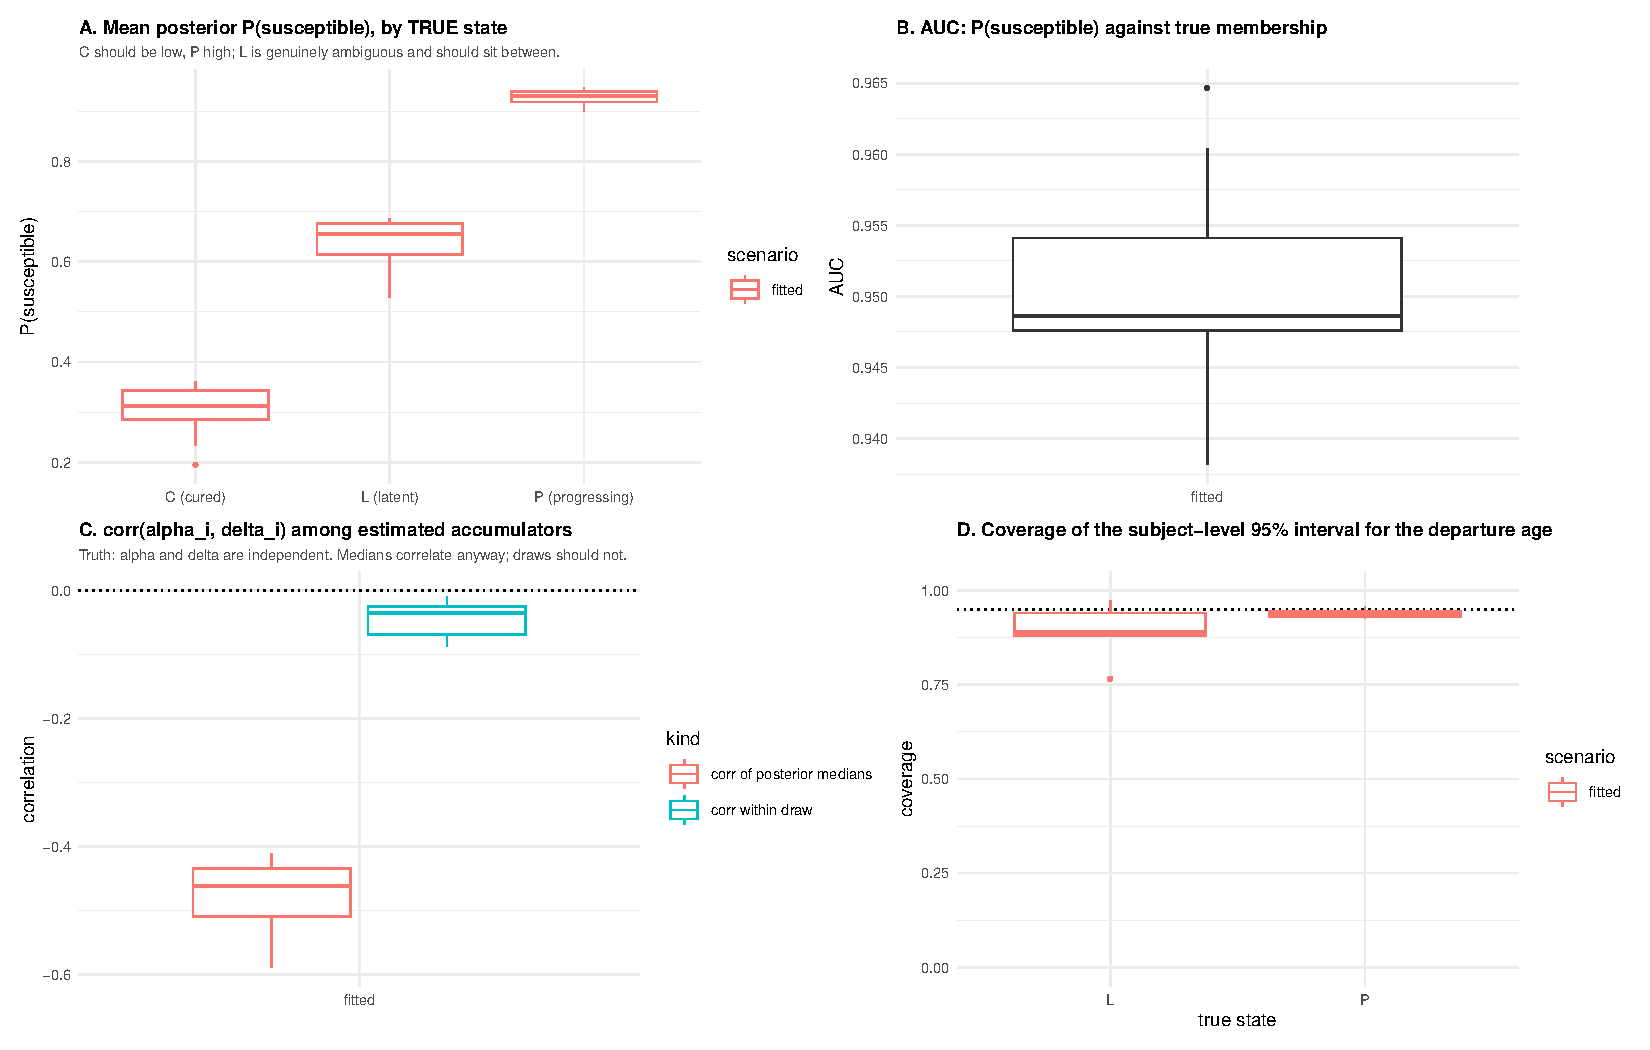
\includegraphics[width=\textwidth]{../figures/sim/full/fig_sim4_subjects.pdf}
\caption{Subject-level recovery across the 8 replicates. (A) Average probability of being an accumulator, by true state. (B) AUC. (C) The correlation between departure age and speed computed two ways; the truth is zero. (D) Coverage of the departure-age interval for subjects who have and have not yet started.}
\end{figure}

%=====================================================================
\section{What this means for the real-data results}

\begin{center}
\small
\begin{tabularx}{\textwidth}{@{}l X@{}}
\toprule
Real-data claim & What the simulation says \\
\midrule
APOE4 strongly raises the odds of ever accumulating & Supported, and probably understated: the estimate is pulled about 23\% toward 1 by the prior. \\
APOE4 brings onset forward, time ratio 0.73 & Recovered without detectable bias; intervals honest. \\
APOE4 has little effect on speed, rate ratio covers 1 & Recovered without detectable bias in this scenario. Whether a real speed effect could be mistaken for an onset effect needs the \code{rate\_only} scenario. \\
Cure fractions of about 41\% and 12\% & The gap between them is somewhat understated, for the same prior reason. \\
Crossing ages 77.5 and 65.1, gap 12.4 years & Recovered to within about a year; the non-carrier age may run slightly high. \\
Per-subject onset ages & Reliable to about $\pm 6$ years for people already accumulating; much less so for people not yet started. \\
\bottomrule
\end{tabularx}
\end{center}

%=====================================================================
\section{Limitations}

\begin{enumerate}
  \item \textbf{Eight replicates.} Enough to find the odds-ratio bias, which is more than 10 Monte Carlo SEs, and to check pooled coverage. Not enough to detect biases under about 2 Monte Carlo SEs, or to judge coverage for any one quantity.
  \item \textbf{One scenario.} Only \code{fitted} has been run. The most important remaining test, whether the model can tell a speed effect from an onset effect, is \code{rate\_only}.
  \item \textbf{A best case.} The data come from the model itself, so model misspecification is absent by construction.
  \item \textbf{Chain length.} 20,000 iterations per chain is borderline for the slowest parameters. One replicate had an R-hat of 1.12, but the misses do not cluster there.
\end{enumerate}

%=====================================================================
\section{Recommended next steps}

\begin{enumerate}
  \item \textbf{Refit the real data with a wider prior on the susceptibility effects}, for example Normal(0, $1^2$) or Normal(0, $1.5^2$) on $\varphi_2$ and $\varphi_3$, and report how the APOE4 odds ratio and cure fractions move. This is a prior-sensitivity analysis, and the simulation shows it is needed. The prior SD is set on the line \code{phi[q] \textasciitilde{} dnorm(0, sd = 0.5)} in \code{R/04\_model.R}.
  \item \textbf{Run the \code{rate\_only} scenario} at the full design, 8 replicates at a time:
\begin{verbatim}
run_simulation("full", scenarios = "rate_only", n_iter = 20000, n_rep = 8)
\end{verbatim}
  \item \textbf{Add \code{fitted} replicates} to firm up the smaller findings, especially the crossing ages and the transit budget. Running with \code{n\_rep = 16} adds 8 more and skips the ones already done.
\end{enumerate}

%=====================================================================
\Needspace{16\baselineskip}
\section{Reproducing this report}

From the project root:

\begin{verbatim}
Rscript -e 'source("run_simulation.R"); summarise_sim("full")'
Rscript sim_results_full/analyse.R
Rscript sim_results_full/tables.R
\end{verbatim}

\code{analyse.R} writes these to \code{sim\_results\_full/}, along with the three figures:
\begin{itemize}
  \item \code{performance\_detailed.csv}: one row per quantity, the table in Section 3;
  \item \code{per\_replicate\_estimands.csv}: every estimate, interval, posterior SD and $z$, per replicate;
  \item \code{prior\_shrinkage.csv}: the shrinkage table;
  \item \code{subject\_level\_per\_rep.csv}: the subject-level measures, per replicate.
\end{itemize}
\code{tables.R} turns those files into the tables above. Rerunning both after adding replicates updates every number.

\end{document}
